\documentclass[11pt]{article}

\usepackage[T1]{fontenc}
\usepackage{mathpazo}
\usepackage{amsmath,amssymb}
\usepackage[margin=1.15in]{geometry}
\usepackage{setspace}
\usepackage{tikz}
\usetikzlibrary{arrows.meta,positioning,calc}
\tikzset{
  box/.style={draw, rounded corners=2pt, align=center, font=\small, inner sep=4pt, text width=2.5cm, minimum height=0.9cm},
  wide/.style={box, text width=3.6cm},
  rep/.style={box, very thick, text width=7.0cm},
  unrep/.style={box, dashed, text width=7.0cm},
  arr/.style={-{Stealth[length=2mm]}, thick},
  darr/.style={-{Stealth[length=2mm]}, thick, dashed},
  lab/.style={font=\scriptsize, align=center}
}
\usepackage[colorlinks=true,linkcolor=black,citecolor=black,urlcolor=black]{hyperref}

\setstretch{1.08}
\setlength{\parindent}{1.4em}
\setlength{\parskip}{0.2em}

\title{What a Network Edit Licenses\\[0.4em]\large Reading, Constructing, and Repairing Trained Networks Through Their Parameters}
\author{Flyxion\\Independent Researcher}
\date{November 2026}

\begin{document}

\maketitle

\begin{abstract}
\noindent Recent work reports that a general-purpose language model can read neural network weights supplied as text and write or edit them to meet a natural-language specification, in some cases without gradient descent and without environment feedback. This essay examines that proposal, called weight-space programming, through the distinction between a network's disposition space and the trajectories it realizes, and it classifies each reported intervention by its purpose and by its means. It argues that the reported results combine three kinds of claim with different warrants: structural recognition, construction of a network from a specification, and repair of an existing network. The reading results support structural recognition and show that one tested procedure failed to infer contextual behavior from weights alone. The construction results support the translation of specifications into parameters and do not isolate parameters as a medium, since the comparison with trained policies confounds information access with method. The repair results support the removal of a diagnosed pathology in one model, and the budget pattern, the unmatched baselines, and the small parameter footprint leave open how much is attributable to interpreting weights, to evaluation-guided search, or to the generic effect of a good intervention. The essay proposes a parameter-access ablation to test whether access to parameter values adds value beyond behavioral diagnosis, argues that an explanation attached to a successful edit proposes an intervention profile whose evidential warrant depends on discriminating tests, sketches a use of diagnostic records for locating recurring failures of the models themselves, and keeps its own conclusions bounded by the reported protocols.
\end{abstract}

\newpage

\section{Introduction}

The proposal that a language model can program in weight space has an appealing simplicity. A trained network is a list of numbers, a language model reads lists of numbers, and so a language model might read what a network computes and write what a network should compute, in the way that it already reads and writes code. The post that develops this proposal reports experiments in which a frontier model, referred to there as Astra, identifies which game a policy network was trained on, names the language on which a transformer was trained when given only its middle blocks, repairs a failing control policy by editing a few percent of its weights, writes small game-playing networks from all-zero weights in a single reply, builds a larger board-game network with tool assistance and a budget of forward passes, and removes a looping pathology from a small language model by subtracting one direction from the output weights of two layers \cite{takehi2026}. The authors describe the results as very early, describe the approach as reasoning-driven optimization that proceeds without an optimizer or gradient descent, and present the further applications they anticipate, including auditing networks for backdoors without evaluating them, steering capabilities without data, and recursive self-improvement, as possibilities and not as demonstrated results.

The post is forthcoming about its limits. It reports that the model failed to identify a sycophantic fine-tune from weights alone in every attempt, that its interpretations were sometimes partial, that its attempt to improve a second small language model produced no established gain, and that the Qwen repair depended on the budget of forward passes. It also draws a distinction that this essay shares, between removing a loop that stops a model from finishing answers it could already work out and making a model better at mathematics. These admissions make the results easier to evaluate, and they suggest that the productive question is not whether the results are impressive but what each result licenses. A reading licenses a claim about what a network does, or about what a particular reader can extract from it. A construction licenses a claim about what a model can build from a specification. A repair licenses a claim about what a model can fix. The evidence conditions differ, and the summary description of the proposal runs them together.

Section 2 summarizes the reported results. Section 3 introduces the distinction between a network's disposition space and the trajectories it realizes and applies it to the reading experiments. Section 4 classifies the interventions by purpose and by means. Sections 5 and 6 examine construction and repair and state the baselines and controls needed to attribute the results to interpretation of weights specifically. Section 7 argues that an explanation attached to an edit proposes an intervention profile whose evidential warrant depends on discriminating tests. Section 8 considers the anticipated applications, Section 9 offers a further application to maintenance and, as a possible use of diagnostic records, to locating recurring failures of the models themselves, and Section 10 states design requirements for the benchmark that the authors say they are building. The essay addresses the claims as the post presents them and does not examine the released logs, and the figures cited are those reported in the post. The framework on which the essay draws is cited from unpublished manuscripts for its vocabulary and formal development, and not for any empirical claim.

\section{The Reported Results}

The reading experiments begin with four policies trained by proximal policy optimization on a shared grid with identical input channels, actions, and dimensions \cite{schulman2017}. Given the weights as text, with no tools and no list of candidate games, the model named the correct game in all four cases, citing features such as the concentration of first-layer input weights along one row of the grid and the differentiation of the output weights for left and right. Three small diffusion models that generate filled shapes were read without tools or forward passes, and the model identified each shape but described each as an outline, which the authors take as evidence that it read the structure of the weights and did not compute a forward pass. Three character-level transformers trained on Python, romanized Japanese, and English were presented with only their four middle blocks, with embeddings and output layers removed. The model could analyze the weights with Python but could not run the network. It named the training language in every case across two attempts and named as copying heads exactly those heads that a measurement on repeated random strings identified, by a method that the authors note is close to a known analysis of transformer circuits \cite{elhage2021}. The failure case is a pair of fine-tuned small language models, one trained toward correct answers and the other toward the answers that users suggest, with the input embeddings and output layers frozen during fine-tuning. From the weights alone the model failed to identify the sycophant in all four attempts. When it was allowed to inspect attention patterns on texts that it wrote, without seeing outputs, it identified the sycophant in all three pairs and located heads that attend to the user's suggested answer in the sycophantic model, while qualifying its own conclusion as evidence for proposal-biased selection and not for a dedicated agreement detector.

The repair and writing experiments include a policy for a ramp-climbing task that had converged on driving straight at the ramp and never succeeding. Given the weights, a scene description, and one recorded episode, the model explained the failure and wrote an edit in one reply, with no tools, that changed about 3.5 percent of the weights and produced success in all 1,024 test episodes. In the account the post gives, the edit adds a small separate path through a few units per layer that reverses the car, commits to a launch, and switches off once the obstacle is cleared. In a second experiment the model wrote small networks for three arcade games from all-zero weights, given the rules, the source code, the input and output layout, and the scoring method, with no data, tools, or rollouts. The written networks scored 517.4 against 25.3 for the trained policy at the larger of two training budgets on one game, 53.1 against 88.9 on a second, and 53.2 against 55.2 on a third, and they exceeded the policy at the smaller budget on all three. In the tool-assisted experiments the model built a board-game network with about 1.5 million weights, using a Python sandbox in which it could edit tensors but not run the network, and a budget of up to 50 forward passes. The post reports that with no passes the written network won more than half its games against two smaller trained networks, and that with passes the model plays practice games, examines losses, revises the part of the network responsible, and keeps a change only if it wins more. In a language-model experiment the model subtracted one direction from 64 output columns in each of two layers of a 0.8-billion-parameter model whose reasoning frequently looped, changing 131,072 weights. At 10, 25, and 50 forward passes the MATH-500 accuracy was 12.3, 14.1, and 48.1 percent against a base of 7.9, and the share of answers reaching the token limit was 87.2, 86.4, and 33.1 percent against 93.0. Instruction following on IFEval rose from 21.0 to 49.0, 39.9, and 62.3 percent across the same budgets. A final attempt on a second small model that rarely loops produced no established gain, and the authors conclude that editing can remove an obstacle that hides an ability but cannot add an ability the model lacks.

\section{Weights as a Disposition Space}

A trained network is, in the vocabulary of the continuation framework, a persistent disposition space and not a behavior \cite{flyxion2026continuation}. The weights fix which input-output continuations are available, and the trajectory that is realized at a given moment depends on the input and on whatever state and decoding procedure intervene. The framework separates the persistent space of dispositions, a fast organizing variable that selects within it, and the instantaneous state and trajectory over an interval, because properties of one level do not follow from properties of the level beneath it without a stated computation. Two things should be kept apart when applying this to reading. Without a specified input, state, and decoding procedure, the disposition space does not determine a trajectory, and this is a missing contextual specification. With all of these fixed, the weights determine the output or its distribution, and a failure to infer a property of the behavior is then a limit on the reader and the protocol, and not an indeterminacy in the parameters. Figure~\ref{fig:disposition} summarizes the two routes by which a property can be read.

\begin{figure}[htbp]
\centering
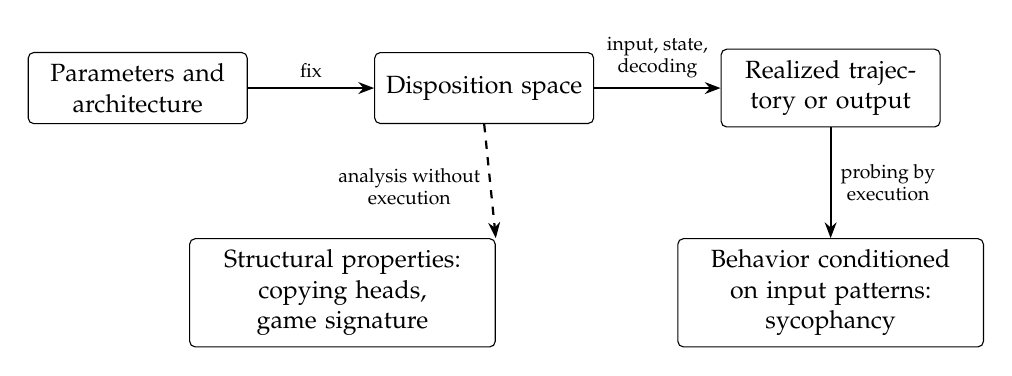
\begin{tikzpicture}
\node[box] (theta) at (0,0) {Parameters and architecture};
\node[box] (S) at (4.4,0) {Disposition space};
\node[box] (T) at (8.8,0) {Realized trajectory or output};
\draw[arr] (theta) -- node[lab, above] {fix} (S);
\draw[arr] (S) -- node[lab, above] {input, state,\\decoding} (T);
\node[wide] (P1) at (2.6,-2.6) {Structural properties:\\copying heads, game signature};
\node[wide] (P2) at (8.8,-2.6) {Behavior conditioned on input patterns:\\sycophancy};
\draw[darr] (S.south) -- node[lab, left, pos=0.55] {analysis without\\execution} (P1.north east);
\draw[arr] (T.south) -- node[lab, right, pos=0.5] {probing by\\execution} (P2.north);
\end{tikzpicture}
\caption{Reading as extraction from a disposition space. Analysis without execution recovered structural properties that the weights carry directly. For behavior conditioned on an input pattern, the reported sycophancy experiment succeeded only when the model could probe the networks by execution.}
\label{fig:disposition}
\end{figure}

The reading experiments sort into questions that differ in how directly the weights carry the property sought. The identification of copying heads is a structural recovery. The composition of query, key, value, and output matrices across layers is an analysis of weights, and the post's report that the model recovered it matches a measurement made by running the network on inputs the model never saw. The identification of a game from a policy network is a recognition task in which the model was not given the candidates, which makes the recognition problem less constrained than a closed choice would be. The evaluation does contain only four networks with distinctive spatial signatures, and it does not test discrimination among closely related tasks, so the result establishes zero-shot recognition of distinctive structure and leaves open how it scales as signatures become similar. The question of which of two fine-tuned networks is sycophantic concerns behavior conditioned on a specific input pattern, namely a user's suggestion of an answer, and the weights carry it through the composition of embeddings and attention circuits across many layers.

On the sycophantic pair, the tested procedure failed from weights alone in four attempts and succeeded when the model could write texts and inspect attention patterns on them. The change is from analysis without execution to sampling trajectories from the network, and the reported success is evidence that, for this behavior and this reader, the route through execution worked where static analysis did not. It does not show that the weights underdetermine the behavior, and it does not establish a general boundary between structural reading and behavioral reading, since one unsuccessful discrimination by one reader under one protocol is a limit of that protocol. What it does show is that the reported evidence for reading is strongest at the structural end and, for contextual behavior, depends on probing. The post's own description of the model as natively reading weights is accurate for structure that the experiments verified against measurement.

The consequence for the proposed application to security is that the application is untested and not refuted. A backdoor is a behavior conditioned on a trigger, and the property that makes it a backdoor is that its targeted effect depends on a trigger and may escape ordinary evaluation. The only reported attempt to infer an input-conditioned behavior from weights alone failed, and the success that followed used execution on texts the model wrote. Whether other readers or protocols can infer trigger-conditioned behavior from weights alone is an open question, and an audit of this kind would need interventions that test the readings, as the successful sycophancy procedure did. The earlier analysis of agentic backdoors in terms of admissibility distinguished a behavior's being justified by an account from its being admissible given the structure that produces it \cite{flyxion2026permissions}, and the same distinction applies to a reading of weights: an account that sounds coherent does not settle what the network will do.

\section{Purpose and Means}

The admissibility framework classifies operations on a system's admissibility structure. An operation is interrogative if it reads the structure without changing it and modificatory if it writes to it. Among modificatory operations it distinguishes constitutive operations, which build structure not previously present, regulatory operations, which reshape how existing structure is used, and restorative operations, which recover structure that has been degraded. The weight-space experiments suggest that purpose and means should be classified separately, since an intervention can serve one kind of purpose by means of another. Figure~\ref{fig:purposemeans} places the reported interventions on the two axes.

\begin{figure}[htbp]
\centering
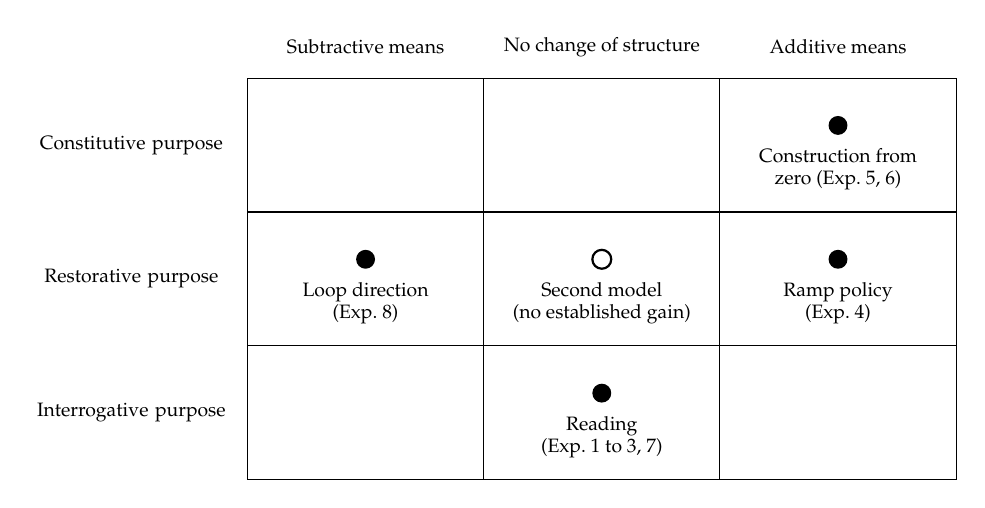
\begin{tikzpicture}
\foreach \x in {-1.5,1.5,4.5,7.5} \draw (\x,-0.85) -- (\x,4.25);
\foreach \y in {-0.85,0.85,2.55,4.25} \draw (-1.5,\y) -- (7.5,\y);
\node[lab] at (0,4.65) {Subtractive means};
\node[lab] at (3,4.65) {No change of structure};
\node[lab] at (6,4.65) {Additive means};
\node[lab, anchor=east, text width=2.4cm] at (-1.65,0) {Interrogative purpose};
\node[lab, anchor=east, text width=2.4cm] at (-1.65,1.7) {Restorative purpose};
\node[lab, anchor=east, text width=2.4cm] at (-1.65,3.4) {Constitutive purpose};
\fill (3,0.25) circle (0.12); \node[lab, below=2pt] at (3,0.15) {Reading\\(Exp.\ 1 to 3, 7)};
\fill (6,3.65) circle (0.12); \node[lab, below=2pt] at (6,3.55) {Construction from\\zero (Exp.\ 5, 6)};
\fill (6,1.95) circle (0.12); \node[lab, below=2pt] at (6,1.85) {Ramp policy\\(Exp.\ 4)};
\fill (0,1.95) circle (0.12); \node[lab, below=2pt] at (0,1.85) {Loop direction\\(Exp.\ 8)};
\draw[thick] (3,1.95) circle (0.12); \node[lab, below=2pt] at (3,1.85) {Second model\\(no established gain)};
\end{tikzpicture}
\caption{Reported interventions classified by purpose and by means. Filled markers show a reported success or gain, and the hollow marker shows an attempt without an established gain. The ramp edit pairs a restorative purpose with additive means, and the loop edit pairs the same purpose with subtractive means.}
\label{fig:purposemeans}
\end{figure}

The reading experiments are interrogative. The construction from all-zero weights is constitutive in both purpose and means. An all-zero network still implements a function, depending on its architecture and its fixed components, and that function may be constant or useless for the task, so the relevant claim is narrower than that the initial network contains nothing. It is that the task-specific controller was not already implemented in the initial parameter configuration, and the writer supplies it. The ramp repair separates purpose from means clearly. Its purpose is restorative, in that the network was meant to solve the task and had converged on a local minimum. Its means are constitutive, in that the account the post gives is of a new computational path that reverses, launches, and relinquishes control, coupled to the previously trained policy. Successful repair therefore need not consist in uncovering a behavior that the network already implemented, and the case shows why a classification by purpose alone would misdescribe it. The language-model repair has a subtractive means, the removal of a direction from output columns, and a purpose of recovering the completion of answers the model might otherwise finish, and it fits the restorative description better, as a hypothesis about what the edit did.

That qualification matters for the conclusion that the authors draw from the second small model, that editing can remove an obstacle but cannot add an ability. A restorative description of an improvement is a functional interpretation that requires evidence, and it is not a mathematical restriction on what a change of parameters can accomplish. An edit changes the input-output function of the network, and whether a capability was independently present before the edit needs independent evidence, such as successful performance under a different elicitation procedure or an intervention that selectively removes the diagnosed obstruction. Under stochastic decoding the mere possibility of an output is too permissive to distinguish ability from inability, since a network may already assign nonzero probability to correct answers while producing them unreliably. The negative result on the second model is compatible with the hypothesis that its failures were ordinary errors without a removable obstruction, and it is reported under different sampling settings and a small number of samples per problem. It does not establish that the model lacked an ability or that editing cannot introduce one, and the ramp repair, which introduces structure, is an example of an edit that does more than remove an obstacle. The distinction the post draws, between letting a model finish answers it could already work out and improving its mathematics, is the right one, and the conclusion should be limited to what the experiment supports, which is that these edits under these budgets did not produce an established improvement in that model.

The classification by meta-depth requires a declared functional boundary. An operation acts at depth zero when it modifies the structure that performs the task and at depth one when it modifies the machinery that performs modifications. Editing another network does not by itself fix the depth, since another network could implement an editor, and editing one's own task-performing parameters need not modify the editing procedure. The proposal of recursive self-improvement requires an improvement to the capacity or process responsible for subsequent improvement, together with evidence that the improved process yields further gains. The reported experiments do not demonstrate improvement of the editing process itself. The bound on attainable depth by resources and by a positive cost per level is a result of the formal development of the framework and applies to such a proposal under that development, and the claim made here is only that no reported experiment reaches the question.

\section{Construction as Compilation}

The construction experiments report the most striking numbers and require the most care in interpretation. A written network that scores about twenty times a trained baseline on one game is a surprising result if the written network and the trained baseline are solutions to the same problem under the same conditions. They are not. The model received the rules of the game, the source code of the environment, the layout of the inputs and outputs, and the scoring method, and the trained baseline received interaction with the environment through reward. The comparison shows a difference in performance between systems with different information and resource histories. It does not apportion that difference among the sample inefficiency of reinforcement learning, access to the specification, the language model's prior training, and the particulars of the implementation. The post reports that the model designed in one game an algorithm whose first layer computes where the ball will land and whose second moves the paddle to that point, which is a program written down and compiled into a small network, and the quality of the result reflects the quality of the program.

The result is therefore best described as a demonstration that a general-purpose model can translate a specification into a weight configuration that implements a designed controller, to the numerical precision that a small tanh network requires. That capacity is not trivial and it is not the same as the capacity to learn a policy. The authors' own table is compatible with the reading that the advantage depends on how easily a controller can be designed from the rules, since the written network is far ahead on the game where such a design is easy and trails or approaches the trained policy on the other two. Two controls would separate the claims. A scripted controller for each game, written by a person or by the model in ordinary code, would give a reference performance for design by reasoning before any weights are written, and it should be described as a reference and not as a ceiling, since a better controller may exist. The clean test of what is specific to realizing a design in parameters holds the designed controller fixed and compares its direct execution with its realization as a network. A gap between separately written code and a separately written network would not measure the loss incurred by compilation, since a network-writer that designs a different and worse algorithm than the code-writer produces a gap that mixes design quality with compilation fidelity. A trained baseline given privileged access to the simulator, for example through model-based search or imitation of the scripted controller, would match the information available to the writer and make the comparison one of methods and not of knowledge. Figure~\ref{fig:construction} contrasts the two designs.

\begin{figure}[htbp]
\centering
\begin{minipage}{\textwidth}
\centering
{\small (a) Designed controller held fixed}\\[2pt]
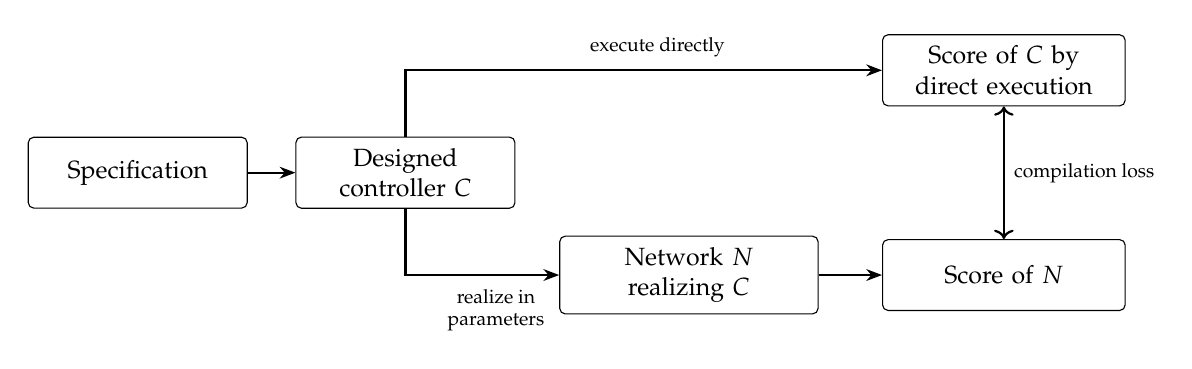
\begin{tikzpicture}
\node[box] (spec) at (0,0) {Specification};
\node[box] (C) at (3.4,0) {Designed controller $C$};
\node[box, text width=3.0cm] (N) at (7.0,-1.3) {Network $N$ realizing $C$};
\node[box, text width=2.8cm] (sC) at (11.0,1.3) {Score of $C$ by direct execution};
\node[box, text width=2.8cm] (sN) at (11.0,-1.3) {Score of $N$};
\draw[arr] (spec) -- (C);
\draw[arr] (C.north) |- (sC.west);
\node[lab] at (6.6,1.6) {execute directly};
\draw[arr] (C.south) |- (N.west);
\node[lab] at (4.55,-1.75) {realize in\\parameters};
\draw[arr] (N) -- (sN);
\draw[<->, thick] (sC.south) -- node[lab, right] {compilation loss} (sN.north);
\end{tikzpicture}\\[10pt]
{\small (b) Separately written code and network}\\[2pt]
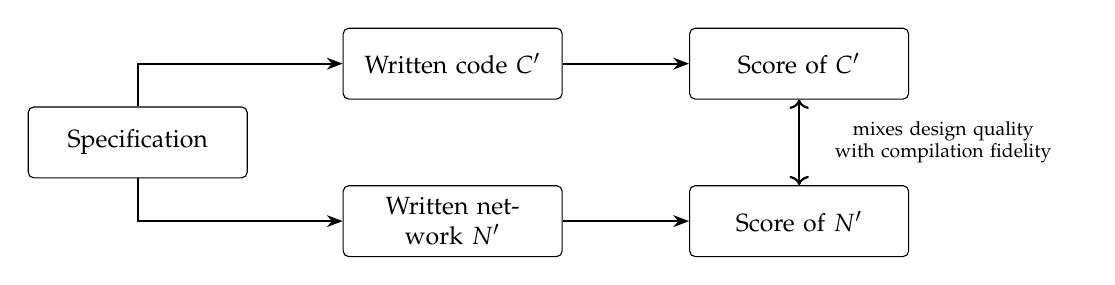
\begin{tikzpicture}
\node[box] (spec) at (0,0) {Specification};
\node[box] (Cp) at (4.0,1.0) {Written code $C'$};
\node[box] (Np) at (4.0,-1.0) {Written network $N'$};
\node[box] (sCp) at (8.4,1.0) {Score of $C'$};
\node[box] (sNp) at (8.4,-1.0) {Score of $N'$};
\draw[arr] (spec.north) |- (Cp.west);
\draw[arr] (spec.south) |- (Np.west);
\draw[arr] (Cp) -- (sCp);
\draw[arr] (Np) -- (sNp);
\draw[<->, thick] (sCp.south) -- node[lab, right, text width=3.4cm] {mixes design quality\\with compilation fidelity} (sNp.north);
\end{tikzpicture}
\end{minipage}
\caption{Controls for construction. In (a) the same designed controller is executed directly and realized in parameters, so the score difference measures the loss incurred by compilation. In (b) the two writers may design different algorithms, so the difference does not.}
\label{fig:construction}
\end{figure}

The result should also be placed against prior work on compiling programs into networks. Methods that compile programs written in a restricted language into transformer weights exist and have been used to test interpretability tools \cite{lindner2023}, and the practice of setting the weights of tiny networks by hand to implement an algorithm is established. The post's related-work section notes this and identifies the novelty as a general-purpose model that performs the translation directly from a natural-language specification and is used as it is. That is a real difference in how the specification is provided and how the translation is performed, and it is a difference of degree from what compilers and people can do for small networks.

The larger experiments raise the question of where the distinctive advantage lies. Because the authors' definition includes tool-assisted tensor editing, the Python sandbox in the board-game experiment is within scope, and what it does not do is separate interpretation from synthesis. The network there was produced by a program of a few hundred lines that describes how to evaluate captures and liberties and emits the layers, and with a budget of forward passes the post describes an explicit iterative procedure in which the model plays practice games, revises the network, and retains changes that improve its results. For that experiment the use of gradient-free optimization is reported and not merely inferred. What remains unresolved is whether the advantage lies in interpreting learned parameters, in synthesizing an algorithm into a fixed architecture, or in using evaluation feedback to improve that synthesis, and the experiments do not factor these apart. Code-mediated construction and direct textual emission of parameters are different implementations that would be worth reporting separately, even though both are within the scope the authors declare.

\section{Repair and Feedback}

The authors describe their approach as reasoning-driven optimization that does not use an optimizer or gradient descent, and the description is accurate to what they say. The question that remains is whether interpretive reasoning about weights improves the proposal and selection of edits relative to other methods under matched information and evaluation budgets. The board-game experiment reports evaluation-guided revision directly. For the language model, the post shows a trajectory of practice accuracy across forward passes and a sequence of edits within each run, and the released logs would establish the sequence of proposals and evaluations. Feedback-assisted editing that may include gradient-free optimization is an accurate description of what the reported procedure shows, and the contribution of the model's reading of the weights to the result is the quantity that has to be measured.

The budget pattern in the language-model experiment is more differentiated than a single threshold. The largest mathematical gains and the substantial suppression of token-limit failures occur at fifty forward passes, with gains on MATH-500 of 4.4 and 6.2 percentage points at the two smaller budgets, against 40.2 points at fifty passes. Instruction following on IFEval, however, already rises sharply at ten passes, falls at twenty-five, and rises again at fifty. The smaller-budget gains on IFEval coexist with little change in the MATH-500 token-limit rate, so the reported results do not establish that every gain has the same termination explanation, and the non-monotone pattern shows that the edits at intermediate budgets have effects that the headline description does not characterize.

Attribution to reading the weights requires comparison with the methods a practitioner would otherwise use. Directional ablation is an established technique in other behavioral domains \cite{arditi2024}, as is steering by adding activation vectors \cite{turner2023}, and contrasting activations on looping and non-looping completions would supply a natural task-specific baseline here, since the looping behavior of small reasoning models is itself documented \cite{pipis2025}. Such methods can be run automatically at a comparable budget of forward passes. A baseline that proposes edits of the same norm and the same number of columns at random tests whether the diagnosed direction has a distinctive effect. A gradient-based fine-tune on the same practice problems at a matched budget of compute tests whether forward passes buy more through reasoning than through the standard method. If the model's edit exceeds these at matched budgets, that establishes the effectiveness of the whole editing procedure, which includes behavioral diagnosis, prior knowledge of looping, and the use of feedback as well as any reading of the weights. If it matches them, the result is evidence that a removable direction exists, which is informative. Isolating the contribution of interpreting the weights requires a further ablation that varies access to parameters while holding the diagnostic evidence and the intervention interface as constant as possible. A full editor can be compared with an editor that receives the same practice outputs and can request the same structured interventions but cannot inspect parameter values. The central question is whether access to parameter values adds measurable value beyond behavioral diagnosis and intervention search. If the parameter-blind editor achieves equivalent performance under a sufficiently powered comparison with matched resources, parameter inspection is not necessary to attain that performance in the tested setting. If the parameter-reading editor performs better, further controls are needed to distinguish interpretive reasoning from other uses of numerical access. Figure~\ref{fig:attribution} shows which input the ablation removes.

\begin{figure}[htbp]
\centering
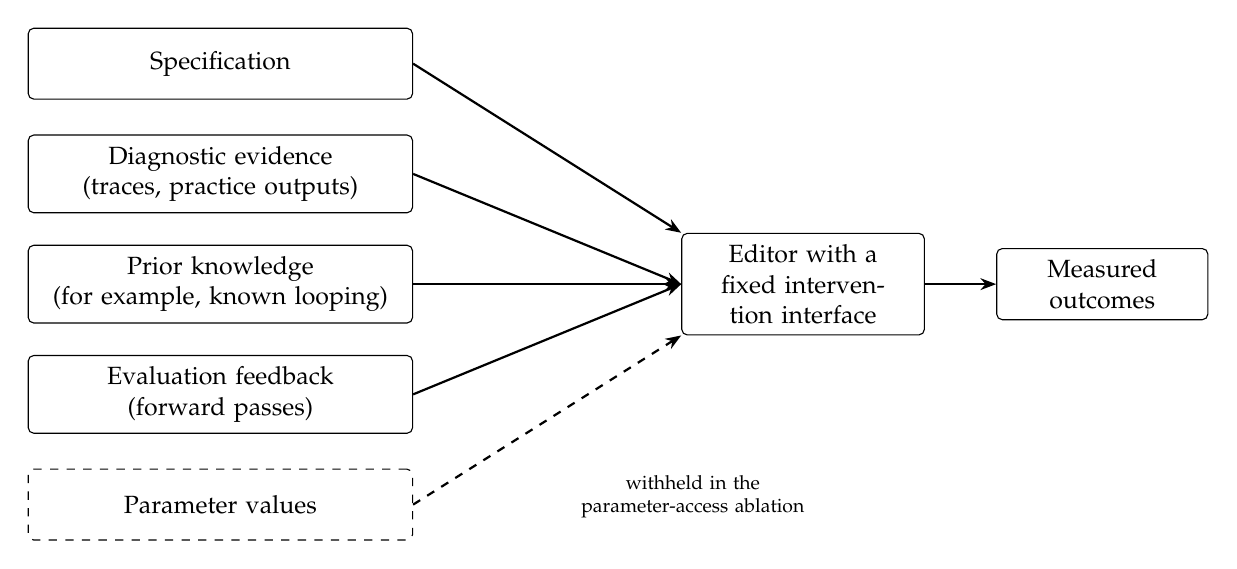
\begin{tikzpicture}
\node[box, text width=4.6cm] (i1) at (0,0) {Specification};
\node[box, text width=4.6cm] (i2) at (0,-1.4) {Diagnostic evidence\\(traces, practice outputs)};
\node[box, text width=4.6cm] (i3) at (0,-2.8) {Prior knowledge\\(for example, known looping)};
\node[box, text width=4.6cm] (i4) at (0,-4.2) {Evaluation feedback\\(forward passes)};
\node[box, text width=4.6cm, dashed] (i5) at (0,-5.6) {Parameter values};
\node[box, text width=2.8cm] (ed) at (7.4,-2.8) {Editor with a fixed intervention interface};
\node[box, text width=2.4cm] (out) at (11.2,-2.8) {Measured outcomes};
\draw[arr] (i1.east) -- (ed.north west);
\draw[arr] (i2.east) -- (ed.west);
\draw[arr] (i3.east) -- (ed.west);
\draw[arr] (i4.east) -- (ed.west);
\draw[darr] (i5.east) -- (ed.south west);
\node[lab, text width=3.4cm] at (6.0,-5.5) {withheld in the\\parameter-access ablation};
\draw[arr] (ed) -- (out);
\end{tikzpicture}
\caption{Sources of information and assistance available to an editor. The parameter-access ablation withholds only the dashed input, holding the diagnostic evidence, the intervention interface, and the resources, including editor inference and tool use, as constant as possible.}
\label{fig:attribution}
\end{figure}

The evaluation protocol deserves attention as well. The base model reached the token limit on most MATH-500 problems under the sampling configuration used, so termination is a major determinant of measured accuracy, while the relation between reaching the limit and receiving a correct score depends on the evaluation procedure. The post marks the distinction between loop removal and mathematical improvement, and the aggregate gain mixes the two. Reporting completion rate and accuracy conditional on completion is informative, but conditioning alone does not separate termination improvement from reasoning improvement, because the edit changes which answers complete. A paired analysis on the same problems, especially those that complete under both the base and edited models, with allowance for sampling variability, would support a more careful decomposition.

The claim that the small footprint of the edit allows a fix without damaging the rest of the model needs separate support. Changing 0.016 percent of the parameters establishes numerical sparsity, and it does not establish functional locality. A sparse edit can affect many inputs and capabilities, particularly when it changes an influential direction in a computation shared across tasks. The statement that such edits avoid the forgetting that fine-tuning often produces requires retention evaluations on behaviors unrelated to the repaired pathology, reported together with base-model values. The intervention licenses claims about the outcomes that were measured, and the small parameter footprint supplies no independent warrant for broad preservation.

\section{Explanation and Licence}

Each reported edit is accompanied by an explanation: the policy fails because it converged on a local minimum and the edit supplies a path that switches behavior at the right moment, and the language model loops because a particular direction written by the output weights of two layers drives repetition. An explanation of why an edit works proposes an intervention profile, the class of interventions that it predicts. The edit that is performed is one member of the class, and its success tests the explanation at one point, so the evidential warrant of the explanation extends only as far as discriminating tests support the profile. The post's own reading of the sycophantic pair illustrates the right attitude, since the model reported its conclusion as evidence for proposal-biased selection and not as evidence for a dedicated detector of user agreement.

For the language-model edit, the explanation that a specific direction drives looping has consequences beyond the ablation that was performed, and they can be stated as tests whose expected outcomes are patterns and not categorical. A sufficiency test should amplify or reintroduce the direction within the same model under controlled conditions and ask whether looping increases, treating transplantation into another model as a separate generalization claim, since a direction can contribute causally in one model without inducing looping elsewhere, where its coordinates and the surrounding circuitry differ. A specificity test should compare the diagnosed direction with matched random directions of the same norm. Random ablations need not leave behavior unchanged, and the relevant question is whether the diagnosed direction has a distinctive effect relative to the matched controls. A dose-response test should vary the scale of the edit and compare the observed pattern with the pattern that the explanation predicts, which need not be monotone and may involve thresholds. Pre-registering the predicted shape, for example monotone up to saturation or a threshold at a stated scale, is what makes the test discriminating, since a test that admits any pattern has no force. The effects at the two layers should be reported both separately and jointly, because the contribution of one component of a joint intervention depends on what else has been changed, and the effect of removing a direction in one layer in the presence of the other is not the intrinsic contribution of that layer \cite{flyxion2026increments}. The post does not report these tests. The reported intervention supports a causal role for the direction under this protocol, in reducing looping and improving the measured outcomes. It does not by itself establish a complete mechanism, a unique cause, or an account of how the direction produces repetition. Figure~\ref{fig:profile} depicts the profile.

\begin{figure}[htbp]
\centering
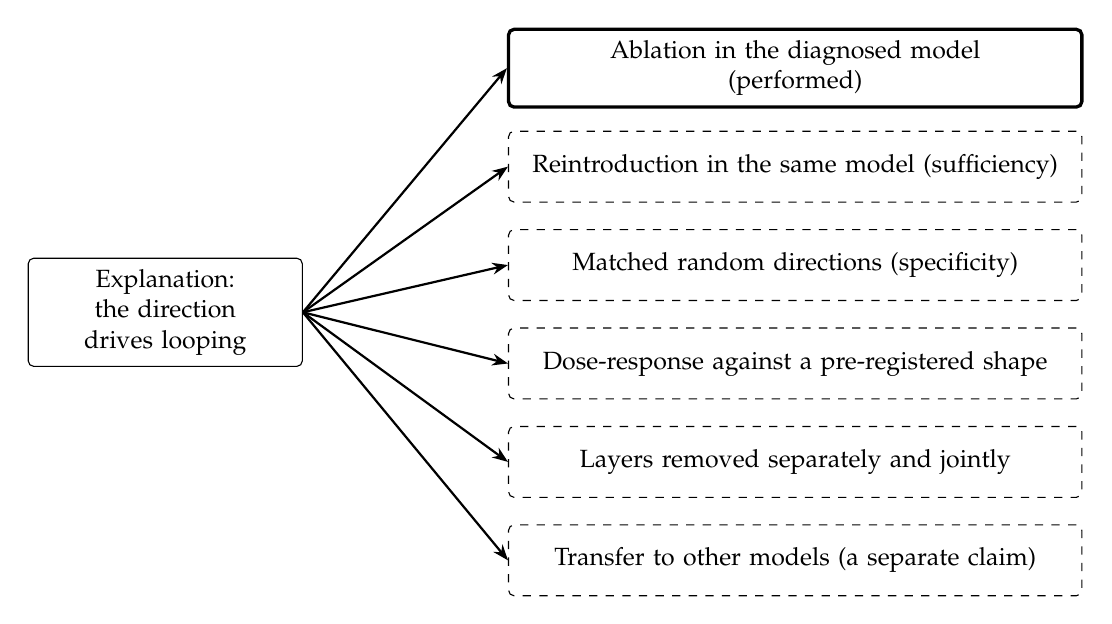
\begin{tikzpicture}
\node[box, text width=3.2cm] (E) at (0,0) {Explanation:\\the direction drives looping};
\node[rep] (a) at (8.0,3.1) {Ablation in the diagnosed model\\(performed)};
\node[unrep] (b) at (8.0,1.85) {Reintroduction in the same model (sufficiency)};
\node[unrep] (c) at (8.0,0.6) {Matched random directions (specificity)};
\node[unrep] (d) at (8.0,-0.65) {Dose-response against a pre-registered shape};
\node[unrep] (e) at (8.0,-1.9) {Layers removed separately and jointly};
\node[unrep] (f) at (8.0,-3.15) {Transfer to other models (a separate claim)};
\foreach \n in {a,b,c,d,e,f} \draw[arr] (E.east) -- (\n.west);
\end{tikzpicture}
\caption{An explanation proposes an intervention profile. The solid border marks the one intervention performed and reported, and dashed borders mark tests that the post does not report. The warrant of the explanation extends only as far as discriminating tests support the profile.}
\label{fig:profile}
\end{figure}

The same point applies to the reading results. The account of why a network corresponds to a particular game or why a head is a copying head is validated, in the post, against a measurement that the model did not see, and this is the right form of validation. It establishes that the account was correct about the property that was measured, and it does not establish that the reasoning behind it was the reasoning the account describes. The shape-drawing result, in which each filled shape was described as an outline, is a useful reminder that a reading can be right about structure and wrong about the behavior that the structure produces. A fluent explanation is a hypothesis that stands in need of intervention, and the quality of the explanation as prose is independent of its evidential standing.

\section{Anticipated Applications and Their Evidential Reach}

The post anticipates several applications, and the sorting by what the reported evidence reaches follows from the preceding sections. The application to auditing for backdoors by reading weights is untested for trigger-conditioned behavior, and the reported failure on the sycophantic pair is the nearest evidence. The application to reducing optimization cost by initializing a model in one shot from a specification, in place of curating data and running training, depends on the comparison with trained baselines under matched information, which Section 5 shows is not yet available. The application to steering capabilities and unlearning without data has support in the repair of a diagnosed pathology in one model, and it needs retention evaluations before the claim of avoiding forgetting can be made, and the negative result on the second model limits the claim to what was tried and does not settle that capabilities cannot be added. The application to merging models by grafting circuits across architectures is a constitutive operation at a scale beyond any reported experiment and has no direct evidence. The application to recursive self-improvement requires improvement of the process responsible for subsequent improvement, which no reported experiment demonstrates.

What the evidence does support can be stated positively and within its protocols. A general-purpose model can emit numerically meaningful weights for small networks from a specification, including specifications that require it to design a controller. It can recognize distinctive structure in small trained networks zero-shot, including structures such as copying heads that match independent measurement. With a budget of forward passes it can diagnose and remove a specific pathology in one language model, with large gains on the reported benchmarks at the largest budget and smaller or non-monotone gains at smaller budgets. In one tested procedure it did not infer a contextual behavior from weights alone, and in one tested model its edits did not produce an established gain. These are substantive results that describe a capable tool for construction from specifications and for repair, and the broader claims about generality, security, and self-improvement are conjectures that further experiments could test.

\section{A Further Application: Maintenance and Diagnostic Records}

The applications that the post anticipates concern the development of models. A further application, offered here as a possibility and not as a result, concerns maintenance. Many small neural controllers are embedded in industrial and medical devices, and some of them have outlived the training data, the software pipeline, and the institutional knowledge that produced them. Such a controller may work under ordinary conditions and fail in one particular situation, for example because a replacement sensor has a different response curve, a motor has developed a dead zone, or an installation has changed the geometry that the controller encounters. Retraining may be impossible, and replacing the controller with a larger model may exceed the memory and inference budget of the hardware. A technician could supply the parameters, the device specification, and a recording of the failure, and ask an editor to construct a narrowly targeted correction inside the existing network. The ramp experiment is a small demonstration of this pattern, in which an added path supplies the missing maneuver and then returns control to the trained policy, and it was produced in one reply from a diagnostic trace. What it shows is that such a repair can be made in one simulated task. It does not show that repairs of this kind are dependable across realistic operating conditions, and that is the speculative part.

Were such a repair attempted, the requirements that follow from the preceding sections would be demanding. A correction that fixes the fault must preserve behavior elsewhere, and a small parameter footprint cannot establish this. Recorded traces of ordinary operation can support an initial retention check by comparing the controllers' outputs on the same observations. They do not establish preservation of closed-loop outcomes, since a changed action can alter subsequent observations and carry the system beyond the recorded trajectory. Evaluating those outcomes requires interactive testing in a suitable simulator or controlled physical setting. The repair must also be evaluated on variations of the fault that were not used to design it, including different magnitudes of the sensor offset or dead zone, and on interactions with other conditions. Where failure has consequences, the verification that the device class requires would still be needed, and a model's ability to produce a correction is not evidence that the correction meets it. A related use is the translation of a technician's explicit rule, such as reducing speed, waiting, and retrying once when pressure rises while flow falls, into a small controller compatible with hardware that expects network parameters. That is construction from a specification, and the benefit would be the natural-language interface and the avoidance of a redevelopment step, and not the discovery of anything hidden in trained weights. Its test is the fixed-controller comparison of Section 5, in which the rule executed directly is compared with its realization in parameters.

A second possibility turns the method on the models themselves. Successive drafts of an essay, together with the corrections that were given, form a record from which recurring failures of a model might be identified. A revision that carefully distinguishes the predictions generated by an explanation from the claims that evidence warrants may be followed by later drafts that reintroduce the conflated wording. For example, a draft may correctly say that an explanation predicts an effect, and a later draft may say that the explanation shows the effect. Such a recurrence is a candidate diagnostic record, and its interpretation needs care, because it can reflect different failures that call for different repairs. It may reflect stale text that was not updated across sections when one section was revised, which is a failure of consistency in the editing process, or a persistent tendency to collapse prediction into warrant in fluent prose, which would be a reasoning defect. The same holds for corrections of transcription, where a misheard technical term and a correctly received term that a language model normalizes into something more familiar can be different failures, the first an acoustic recognition problem and the second a linguistic expectation overriding the available evidence, and they may call for different repairs. A single error may also involve both weak acoustic evidence and a strong language prior, so the distinction is a diagnostic hypothesis and not an exhaustive division. Preserving the inputs, the intermediate transcripts where the system exposes them, the initial outputs, the corrections, and the subsequent behavior would allow the failure to be located, and a stable defect would show itself by recurring across controlled variations and not in a single passage. If one were found, the repair target would be the preservation of a distinction in unfamiliar arguments, including cases where the misleading formulation sounds persuasive, and the repair would be evaluated on held-out material for the same distinction while other abilities are checked for retention. The evaluation must distinguish preservation of the underlying relation from suppression of particular expressions. It should include unfamiliar formulations of the same error and cases in which the stronger conclusion is warranted, so that improved discrimination is separated from indiscriminate qualification. The reported results do not establish that defects of this abstract kind can be located and repaired through parameters. The proposal is offered because it gives the method a target richer than benchmark scores, and because high performance elsewhere does not cancel a specific defect when the defect concerns a distinction on which the current task depends.

\section{Design Requirements for a Benchmark}

The authors state that they are building a benchmark and harness for weight-space programming, and the analysis above suggests requirements that would allow it to separate the claims. The first is information parity. Each comparison between a written or edited network and a trained one should specify what each method was told, and where the model receives a specification that the trained method does not, a baseline with matched access should be included. The second is the separation of feedback regimes. Results should be reported for zero feedback, for fixed budgets of feedback, and across budgets, with the sequence of proposals and evaluations recorded, so that the contribution of reading can be distinguished from the contribution of search. The third is the inclusion of the standard alternatives at matched budgets: scripted controllers and a fixed designed controller executed directly for construction tasks, and direction ablation, activation steering, random-direction controls, and fine-tuning for repair tasks. The fourth is a parameter-access ablation, comparing a full editor with one that receives the same practice outputs and structured interventions but cannot inspect parameter values, with resources matched to include editor inference and tool use as well as target-model evaluations, since equal forward-pass counts alone need not mean comparable expenditure. The fifth is the pre-registration of explanatory predictions as patterns, so that each reported explanation is accompanied by the interventions it predicts and the outcomes are recorded whether or not they favor it. The sixth is held-out failure modes, so that a repair method is evaluated on obstructions that were not used to design it. The seventh is the decomposition of aggregate gains by paired outcomes on the same problems, reporting completion and conditional accuracy together with sampling variability. The eighth is retention evaluation on behaviors unrelated to the repaired pathology, with base-model values. The ninth is the classification of each intervention by its purpose and by its means. The tenth is the use of models that others can run, so that results can be reproduced and the dependence on any particular frontier model can be measured.

A benchmark that met these requirements would also have the property that its negative results are informative. The failure on the sycophantic pair and the absence of an established gain on the second language model are among the most useful findings in the post because they mark where the tested procedures stop. A benchmark that reports where each procedure stops, with the care that the post gives to those cases, would establish the scope of weight-space programming more securely than any single large result.

\section{Conclusion}

Weight-space programming, as reported, is best understood as a family of interventions on a network's disposition space whose purposes and means should be classified separately. Reading is interrogative and succeeds, in the reported experiments, where the weights carry a distinctive structure that a bounded analysis can extract and verify against measurement, and the one tested procedure for an input-conditioned behavior failed from weights alone and succeeded when it could probe the network by execution. Construction from a specification is constitutive and shows that a general model can translate a designed controller into parameters, though the comparison with trained policies confounds the method with the information it was given and leaves open how much is specific to parameters as a medium. Repair in the reported experiments includes one-shot editing from a diagnostic trace, as in the ramp policy, and iterative editing with evaluation feedback, as in the language model, and its means are constitutive in the first case and subtractive in the second. It shows that a diagnosed obstruction can be located and removed from diagnostic evidence, with or without subsequent evaluation feedback, though it does not yet separate interpretation of the weights from the standard methods that also locate such directions, and a small parameter footprint does not by itself warrant claims of preserved behavior. The explanations attached to the results propose intervention profiles whose evidential warrant depends on discriminating tests, most of which the post does not report. What remains unresolved is the attribution: how much of each outcome is owed to interpreting the weights, and how much to the specification the model was given, the diagnostic evidence it received, and the feedback it used. Resolving that attribution requires controls that vary these sources of information and assistance separately.

\begin{thebibliography}{99}
\small
\setlength{\itemsep}{0pt}

\bibitem{arditi2024} Arditi, A., Obeso, O., Syed, A., Paleka, D., Panickssery, N., Gurnee, W., and Nanda, N. 2024. Refusal in Language Models Is Mediated by a Single Direction. In \emph{Advances in Neural Information Processing Systems} 37.

\bibitem{elhage2021} Elhage, N., Nanda, N., Olsson, C., et al. 2021. A Mathematical Framework for Transformer Circuits. \emph{Transformer Circuits Thread}.

\bibitem{flyxion2026continuation} Flyxion. 2026. Continuation Fields: Waves, Admissibility, and the Selection of Thought. Unpublished monograph.

\bibitem{flyxion2026increments} Flyxion. 2026. Increments Are Not Contributions. Unpublished essay.

\bibitem{flyxion2026permissions} Flyxion. 2026. Reasons Are Not Permissions. Unpublished essay.

\bibitem{lindner2023} Lindner, D., Kram\'ar, J., Farquhar, S., Rahtz, M., McGrath, T., and Mikulik, V. 2023. Tracr: Compiled Transformers as a Laboratory for Interpretability. In \emph{Advances in Neural Information Processing Systems} 36.

\bibitem{pipis2025} Pipis, C., Garg, S., Kontonis, V., Shrivastava, V., Krishnamurthy, A., and Papailiopoulos, D. 2025. Wait, Wait, Wait... Why Do Reasoning Models Loop? arXiv:2512.12895.

\bibitem{schulman2017} Schulman, J., Wolski, F., Dhariwal, P., Radford, A., and Klimov, O. 2017. Proximal Policy Optimization Algorithms. arXiv:1707.06347.

\bibitem{takehi2026} Takehi, R., Teoh, J., Zhang, A., and Khattab, O. 2026. Sparks of Weight-Space Programming: LLMs Can Natively Read and Write Neural Network Weights. Blog post, November 2, 2026. \url{https://rikiyat.github.io/blog/weight-space-programming/}.

\bibitem{turner2023} Turner, A. M., Thiergart, L., Leech, G., Udell, D., Vazquez, J. J., Mini, U., and MacDiarmid, M. 2023. Activation Addition: Steering Language Models Without Optimization. arXiv:2308.10248.

\end{thebibliography}

\end{document}
